\section{Wykorzystane technologie}
Do stworzenia aplikacji wykorzystano wiele technologii, narzędzi deweloperskich oraz technik opisanych w poniższych podrozdziałach.

\subsection{Java 8}
Aplikacja w całości została napisana w języku Java.
Java jest językiem programowania ogólnego przeznaczenia, zorientowanym obiektowo. Posiada obsługę wyjątków oraz naturalne wsparcie dla wielowątkowości, pozwala na szybkie tworzenie wysokopoziomowych programów. Aplikacje napisane w języku Java kompilowane są do kodu bajtowego, który uruchamiany jest przez wirtualną maszynę Javy (JVM), niezależnie od architektury urządzenia.

Dzięki wieloplatformowości stworzony program może być uruchamiany na każdym systemie operacyjnym z wirtualną maszyną Javy.

W projekcie aplikacji wykorzystano język Java w wersji 8. 
Pozwoliło to na użycie w projekcie takich elementów języka, jak: wyrażenia lambda i interfejsy funkcyjne (skracające zapis i zwiększające czytelność kodu) oraz strumieni (stream API) - do szybkiego i przejrzystego przekształcania i filtracji danych.

\subsection{JavaFX}
JavaFX jest platformą do tworzenia aplikacji desktopowych (okienkowych) pisanych w języku Java.
Od wersji 8 JavaFX została właczona do platformy Java Standard Edition.
Jest to nowsze, obecnie zalecane przez firmę {\it Oracle} rozwiązanie do tworzenia aplikacji okienkowych. Nie zaleca się natomiast korzystania z bibliotek {\it AWT} lub {\it Swing} \cite{javafx-replacing-swing}.

Do zbudowania widoków aplikacji wykorzystano specjalny format plików FXML, w którym to JavaFX przechowuje informację o właściwościach komponentów interfejsu użytkownika oraz o ich wzajemnych relacjach.

\subsection{Spring}
\subsubsection{Spring Framework}
Spring jest frameworkiem, który umożliwia w aplikacjach Javy zastosowanie wzorca architektonicznego odwrócenia sterowania (IoC - ang. {\it Inversion of Control}), a w szczególności wstrzykiwania zależności (ang. {\it Dependency Injection}). Pozwala to uniknąć występowania bezpośrednich zależności pomiędzy komponentami oraz umożliwia automatyczne dostarczanie i zarządzanie cyklem życia komponentów aplikacji.

W zaprojektowanej aplikacji Spring jest wykorzystywany m.in. do automatycznego dostarczania współdzielonych danych o parametrach symulacji oraz do zarządzania cyklem życia klas prezenterów i widoków z biblioteki JavaFX.

\subsubsection{Spring Boot}
Spring Boot jest rozwiązaniem przyspieszającym proces konfiguracji, tworzenia oraz uruchamiania aplikacji opartych na Spring Framework.
Jest to zestaw wstępnie skonfigurowanych komponentów, dzięki którym jeszcze łatwiejsze staje się dołączenie nowych bibliotek zewnętrznych do projektu. Celem jest pozbycie się zbędnych konfiguracji w plikach XML a zastąpienie ich domyślnym zestawem konfiguratorów, gdyż większość komponentów w aplikacji zazwyczaj konfigurowana jest w typowy, powtarzalny sposób \cite{docs-springboot}.

Spring Boot dostarcza do aplikacji symulacyjnej wiele zależności do bibliotek (np. logback) oraz dostarcza konfigurację dla systemu budowania Maven.
\subsubsection{Spring Boot JavaFx Support}
{\it Spring Boot JavaFx Support} jest niewielką biblioteką umożliwiającą użycie Spring Boot w jednym projekcie w połączeniu z JavaFx.

\subsection{jUnit i Test-driven development}
jUnit jest frameworkiem do wykonywania testów jednostkowych dla programów napisanych w Javie. Testy jednostkowe weryfikują poprawność działania pojedynczych komponentów aplikacji. Uruchamiane są automatycznie podczas budowania projektu.

W projekcie zastosowano podejście TDD (ang. {\it Test-driven development}) dla procesu rozwoju oprogramowania. Dotyczy to w szczególności rozwoju logiki silnika planowania tras dla algorytmu A* i WHCA*. Algorytm WHCA* jest na tyle złożony, że zdecydowano się najpierw napisać szczególne przypadki testowe, które określały jakie dane wyjściowe (zaplanowane trajektorie) są oczekiwane przy zadanych danych wejśiowych. Dopiero po takim pokryciu testami przystąpiono do implementacji algorytmu. Warunkiem poprawności zaimplementowanego algorytmu było, aby wszystkie testy jednostkowe wykonały się prawidłowo. Na tym właśnie podejściu opiera się proces TDD (ang. {\it Test-driven development}), który jest naturalnie wspierany przez framework jUnit.

Bibliotekę jUnit wykorzystano także do wykonania testów skuteczności algorytmów i wszystkich pozostałych testów opisanych w rozdziale \ref{ch:tests}. Pomimo, że nie jest to typowym zastosowaniem biblioteki jUnit, to jednak umożliwia to wykonanie fragmentów logiki w innych, niestandardowych trybach pracy bez zmiany działania głównej aplikacji w normalnym trybie.

\subsection{Maven}
{\it Apache Maven} jest narzędziem do automatyzacji procesu budowania aplikacji napisanych w języku Java.
Przy pierwszym wykorzystaniu zadeklarowanych bibliotek Maven automatycznie pobiera biblioteki ze swojego repozytorium i rozwiązuje wszystkie brakujące zależności do nich. Użytkownik zatem nie musi martwić się o brakujące biblioteki i o manualne dołaczanie ich do projektu.

Narzędzie to zostało użyte w aplikacji do kompilacji ze źródeł oraz uruchamiania. Konfiguracja procesu budowania dla Maven jest wspomagana przez Spring Boot. Uruchomienie programu z kodów źródłowych następuje po wykonaniu w systemie polecenia: $mvn spring-boot:run$.
Do kompilacji i uruchomienia całej aplikacji wystarczy zatem, aby w systemie operacyjnym było zainstalowane środowisko Java JDK oraz {\it Apache Maven}. Wszystkie potrzebne biblioteki zostaną pobrane automatycznie przez sieć Internet.

\subsection{IntelliJ IDEA}
IntelliJ IDEA jest zintegrowanym środowiskiem deweloperskim przeznaczonym głównie do rozwoju aplikacji w języku Java.
Podczas opracowywania oprogramowania korzystano z wersji IntelliJ IDEA Ultimate 2017.2.6, z licencji studenckiej. Zrzut ekranu podczas pracy ze środowiskiem zaprezentowano na rysunku \ref{fig:app-tech-intellij}.
Środowisko to zapewnia integrację ze wszystkimi technologiami wymienionymi w tym podrozdziale.

Aplikacja była rozwijana i testowana na systemach operacyjnych z jądrem Linux (Arch Linux oraz Debian 9), jednak wszystkie zastosowane narzędzia oraz technologie są wieloplatformowe i z powodzeniem mogą być uruchomione na innych systemach opearcyjnych (np. Windows, macOS)

\begin{figure}
	\centering
	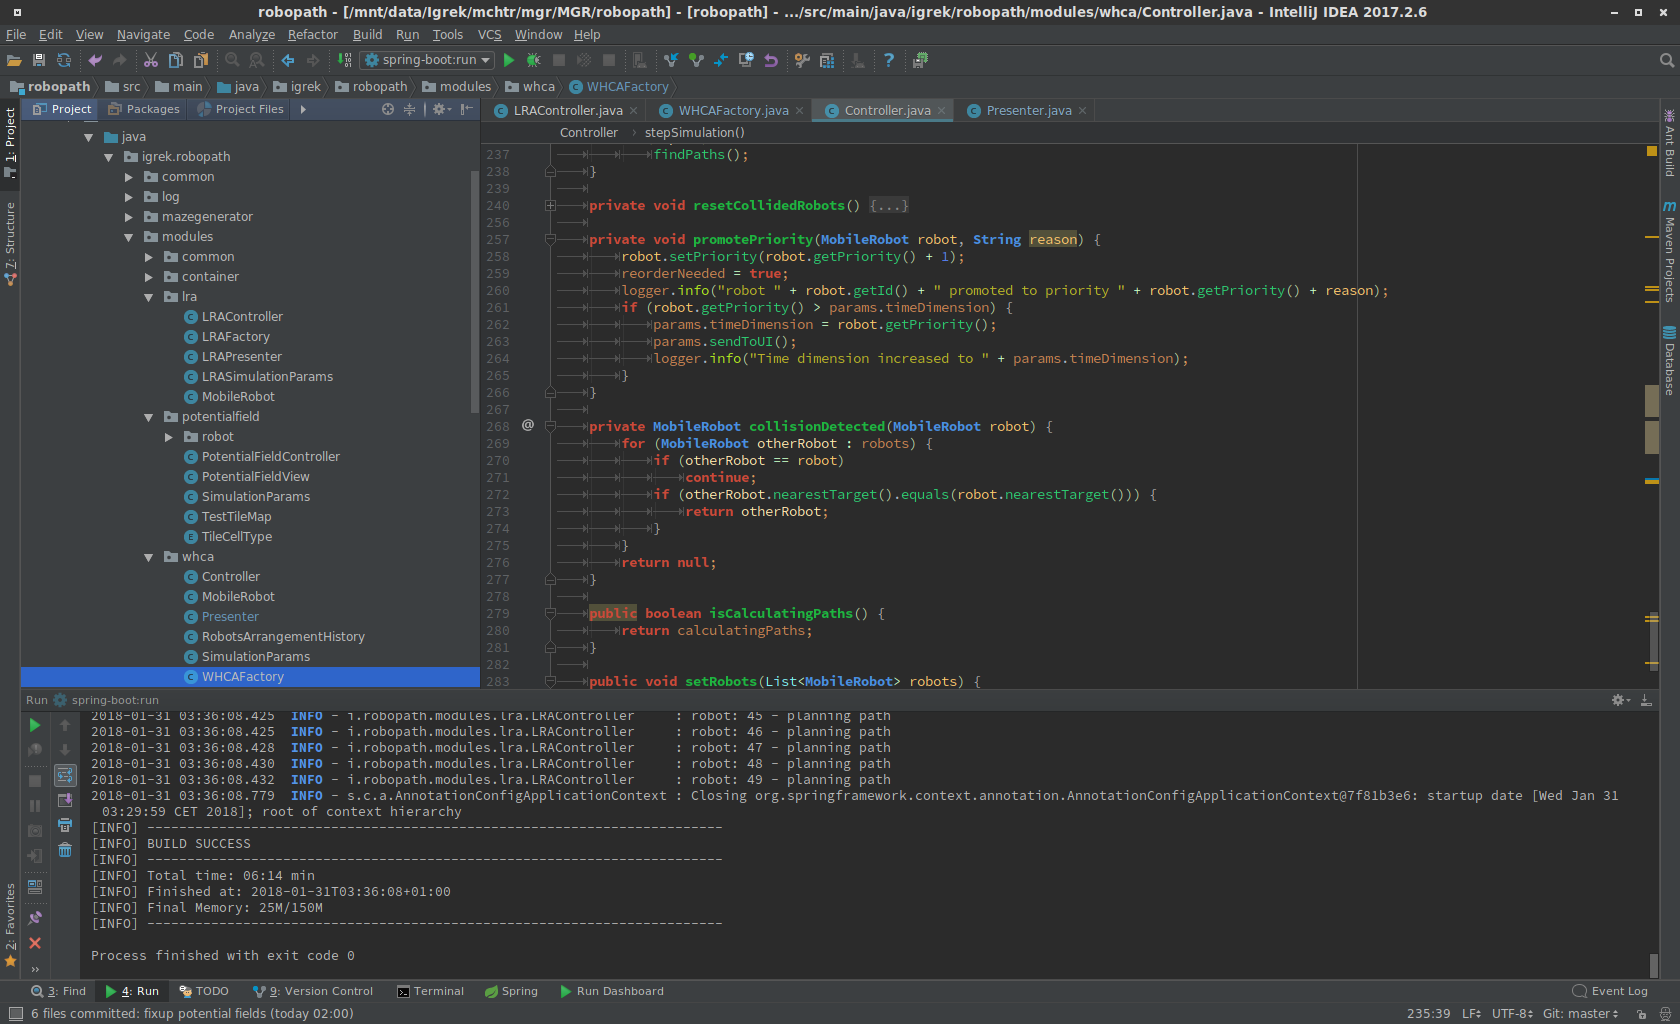
\includegraphics[width=0.9\columnwidth]{img/robopath/intellij}
	\caption{Zrzut ekranu środowiska deweloperskiego Intellij IDEA Ultimate}
	\label{fig:app-tech-intellij}
\end{figure}

\subsection{Pozostałe narzędzia i biblioteki}
\subsubsection{Guava}
Guava jest biblioteką rozwijaną przez Google dostarczającą do Javy m.in. nowe typy kolekcji (struktur danych). W rozwijanej aplikacji wykorzystano ją m.in. do przetwarzania łańcuchów tekstowych.
\subsubsection{git}
Do śledzenia i zapisywania zmian wykorzystano w projekcie system kontroli wersji {\it git}.
Kody źródłowe powstałego programu są ogólnie dostępne w repozytorium git na portalu GitHub:

$TODO$ adres Github
\subsubsection{Logback}
Do zapisu dziennika zdarzeń oraz błędów w aplikacji została wykorzystana biblioteka {\it Logback}, która jest domyślnie dostarczana do aplikacji i skonfigurowana dzięki {\it Spring Boot}.


\section{Struktura aplikacji}
% \subsection{Model-View-Presenter}
Oprogramowanie zostało zorganizowane w architekturę warstwową.
Główny szkielet aplikacji zbudowany jest w oparciu o wzorzec architektoniczny MVP (ang. {\it Model-View-Presenter} - Model-Widok-Prezenter), będący pochodną wzorca MVC (ang. {\it Model-View-Controller}).
Takie podejście zapewnia separację głównej logiki dziedziny programu od warstwy interfejsu użytkownika.

Wybrano podejście MVP, gdyż (w porównaniu do MVC) oferuje ono łatwiejszą testowalność kodu, możliwość "odczepiania" i wymieniania poszczególnych warstw (w celach testowania). Zapewnia to także większą separację modelu z widokiem, które nie muszą "wiedzieć" o sobie, a komunikują się jedynie za pośrednictwem prezentera.

Każdą zaimplementowaną metodę symulacji ruchu robotów zamknięto w osobnych modułach (pakietach). Każdy z tych modułów posiada swoje osobne klasy pochodzące z architektury MVP:
\begin{itemize}
	\item {\bf Model} jest zbiorem klas zajmujących się główną logiką dziedziny aplikacji. Model reprezentowany jest m.in przez klasy odpowiedzialne za reguły poruszania się robotów, obsługę wykonywania kolejnych kroków symulacji, algorytmy planowania trajektorii, kolejkowanie zaplanowanych ruchów, działania na wektorach (w metodzie pól potencjalnych) oraz reprezentację pól na mapie.
	\item {\bf Widok} jest reprezentacją interfejsu użytkownika, który wyświetla dane i kieruje informacje o akcjach użytkownika (zdarzeniach) do prezentera. W tym wypadku instancje widoków generowane są automatycznie przez mechanizmy JavaFX na podstawie ich definicji zapisanych w plikach formatu FXML.
	\item {\bf Prezenter} deleguje dane otrzymane z modelu do widoku, uprzednio przygotowując je do wyświetlenia. Jest w nim zawarta logika warstwy prezentacji.
\end{itemize}

Taka separacja warstw prezentacji od warstwy logiki umożliwia łatwe "odpięcie" logiki od interfejsu użytkownika i wykorzystanie jej do wykonania testów skuteczności metod planowania. Pozwala to wtedy na wykonanie "przyspieszonej" symulacji poprzez sekwencyjne uruchamianie kroków symulacji tak szybko, jak to możliwe, zamiast oczekiwania na wyzwolenie ich przez kolejne cykle zegara.
Klasy modelu były projektowane właśnie z myślą o możliwości wykorzystania ich zarówno w wizualizacji w czasie rzeczywistym, jak i w przyspieszonej symulacji w celu przeprowadzenia testów.

$TODO$
Aplikacja uruchamia planowanie trajektorii w osobnych wątkach w tle, aby nie wpływać na wątek interfejsu użytkownika i uzyskać możliwie płynne animacje. Wymaga to synchronizacji między wątkami, jednak język Java zapewnia stosunkowo łatwą obsługę wątków i synchronizacji sekcji krytycznych. Wątki obliczeń oraz odświeżania interfejsu użytkownika są powtarzane w stałych, zadanych cyklach zegara, które nie są ze sobą zsynchronizowane (nie czekają na siebie), co daje efekt symulacji w czasie rzeczywistym, niezależnie od stanu ukończenia obliczeń.

$TODO$
Klasy serwisów, prezenterów oraz widoków są automatycznie instancjonowane przez Spring Framework. Dzięki wykorzystaniu kontenera IoC (ang. {\it Inversion of Control}) możliwe jest zautomatyzowane wstrzykiwanie zależności (ang. {Dependency Injection}) do poszczególnych instancji.

Do instancjonowania potrzebnych obiektów wykorzystano wzorzec fabryki.

% \section{Dodatkowe funkckjonalności}
% ustawianie random seeda
% działania na wektorach, immutable vector
% heuristic cache
% kolejkowanie ruchów robota
% component scan ze springa - spring boota
% ponowne wykonanie symulacji - te same warunki
% przełaczanie między metodami na zakładkach ?
% resizable window - responsive
% wykonanie symulacji w pojedynczych krokach

\section{Ograniczenia}
W aplikacji zostały wprowadzone pewne uproszczenia, które m.in. przyspieszają i ułatwiają proces obliczeniowy planowania trajektorii dla robotów.
\begin{enumerate}
	\item Założono, że ruch ukośny robota o jedno pole (po przekątnej) trwa tyle samo, co ruch poziomy lub pionowy. Wprowadzono takie przybliżenie ze względu na możliwość ujednolicenia jednostki wymiaru czasu w tablicy rezerwacji pól przez agentów.
	\item Nie uwzględniono czasu obrotu robota podczas zmiany kierunku jazdy. Założono, że czas ten jest zerowy, gdyż celem zaprojektowanego algorytmu było skupienie się na rozwiązaniu innego zagadnienia - problemu zakleszczeń w wąskich gardłach.
\end{enumerate}

% $TODO$ publikacja na GitHub, licencja MIT, filmiki na YT